\documentclass{article}
\usepackage[T1]{fontenc}
\usepackage{lmodern}
\usepackage[utf8]{inputenc}
\usepackage[british]{babel}
\usepackage{geometry}
\usepackage{color}
\usepackage{amsthm}
\usepackage{amsmath,amssymb}
\usepackage{graphicx}
\usepackage{mathtools}
\usepackage{listings}
\usepackage{newlfont}
\usepackage{tikz-cd}

\newcommand{\numberset}{\mathbb}
\newcommand{\N}{\numberset{N}}
\newcommand{\Z}{\numberset{Z}}
\newcommand{\R}{\numberset{R}}
\newcommand{\Q}{\numberset{Q}}
\newcommand{\C}{\numberset{C}}
\newcommand{\K}{\numberset{K}}
\newcommand{\F}{\numberset{F}}
\newcommand{\n}{\mathcal{N}}
\newcommand{\aid}{\mathfrak{a}}
\newcommand{\bid}{\mathfrak{b}}
\newcommand{\pid}{\mathfrak{p}}
\newcommand{\qid}{\mathfrak{q}}
\newcommand{\mi}{\mathfrak{m}}
\newcommand{\I}{\mathbb{I}}
\newcommand{\V}{\mathbb{V}}
\newcommand{\Ps}{\mathbb{P}}

\DeclareMathOperator{\Ima}{Im}
\DeclareMathOperator{\sgn}{sgn}

\newcommand{\exercise}[1]{\noindent {\bf Exercise #1}}

\begin{document}

\title{Algebraic Topology 1 - Assignment 8}

\author{M. Durante, s2303760, Leiden University\\M. Fruttidoro, s2287129, Leiden University\\I. Prosepe, s2290162, Leiden University}

\maketitle


\exercise{1}

$(a)$ First, we give a description of $X$.

It is enough to describe the attaching maps: $f_1:J_1\times\partial D^1\rightarrow X_0$ is constant, as $X_0=\{e_0\}$; $f_2:\partial D^2\rightarrow X_1$ runs along the sides starting from $e_0$, moving along $a$, then $b$, $a^{-1}$, $b^{-1}$, $c$, $d$, $c^{-1}$ and $d^{-1}$, where $x^{-1}$ refers to the 1-cell $x$ with opposite orientation.

By~\cite[cor. 9.6]{sag}, we get that $\tilde{C}_0(X,\Z)=H_0(X_0,X_{-1},\Z)\cong H_0(X_0,\Z)\cong\Z$, $\tilde{C}_1(X,\Z)=H_1(X_1,X_0,\Z)\cong\Z^4$ and $\tilde{C}_2(X,\Z)=H_2(X_2,X_1,\Z)\cong\Z$ while for $n>2$, since $X_{n-1}=X_n=X$, $\tilde{C}_n(X,\Z)=H_n(X_n,X_{n-1},\Z)\cong 0$.

We consider now the sequence $0\rightarrow\tilde{C}_2(X,\Z)\xrightarrow{\tilde{\partial}_2}\tilde{C}_1(X,\Z)\xrightarrow{\tilde{\partial}_1}\tilde{C}_0(X,\Z)\rightarrow 0$.

Trivially, $H_n(X,\Z)\cong H_n(\tilde{C}(X,\Z))\cong 0$ for $n>2$.

Choosing for each $j\in J_n$ a generator $1_n\in H_n(D^n,\partial D^n,\Z)$, the $e^n_j=\chi_j(1_n)$ form a $\Z$-basis of $H_n(X_n,X_{n-1},\Z)$ by~\cite[cor. 10.1]{sag}, hence we may just see where these elements are sent.

By~\cite[thm. 10.4]{sag}, the coefficient $d_{jk}$ in $\tilde{\partial_n}(e^n_j)=\sum_{k\in J_{n-1}} d_{jk}e^{n-1}_k$ is given by $\deg(h_{n-1}\circ q_k\circ q\circ f_n|_{\{j\}\times\partial D^n})$.

Since the degree map is multiplicative, being $f_1|_{\{j\}\times\partial D^1}$ constant and hence of degree 0, $\deg(h_0\circ q_k\circ q\circ f_1|_{\{j\}\times\partial D^1})=\deg(h_0\circ q_k\circ q)\deg(f_1|_{\{j\}\times\partial D^1})=0$, i.e. $\tilde{\partial_1}$ is the zero-map.

It follows that $H_0(X,\Z)\cong\ker(\tilde{\partial}_0)/\Ima(\tilde{\partial}_1)=\Z/0\cong\Z$.

Consider now a loop representing a generator of $H_2(\partial D^2,\Z)$. It wraps $\partial D^2$ once and it is sent by $f_2$ to a loop wrapping $X_1$ like $f_2$ does. Being $X_1\xrightarrow{q} X_1/X_0$ an identity, it doesn't act, while the projection $X_1/X_0\xrightarrow{q'} D^1/\partial D^1\cong S^1$ is s.t. now the image is a loop wrapping $S^1$ multiple times (once for every wrapping of a 1-cell, which are 8), however for every wrapping there is an inverse wrapping, thus the image of the generating loop under $q'\circ q\circ f_2$ is homotopy equivalent to the constant one and $\deg(h_1\circ q'\circ q\circ f_2)=\deg(h_1)\deg(q'\circ q\circ f_2)=0$.
\begin{figure}
  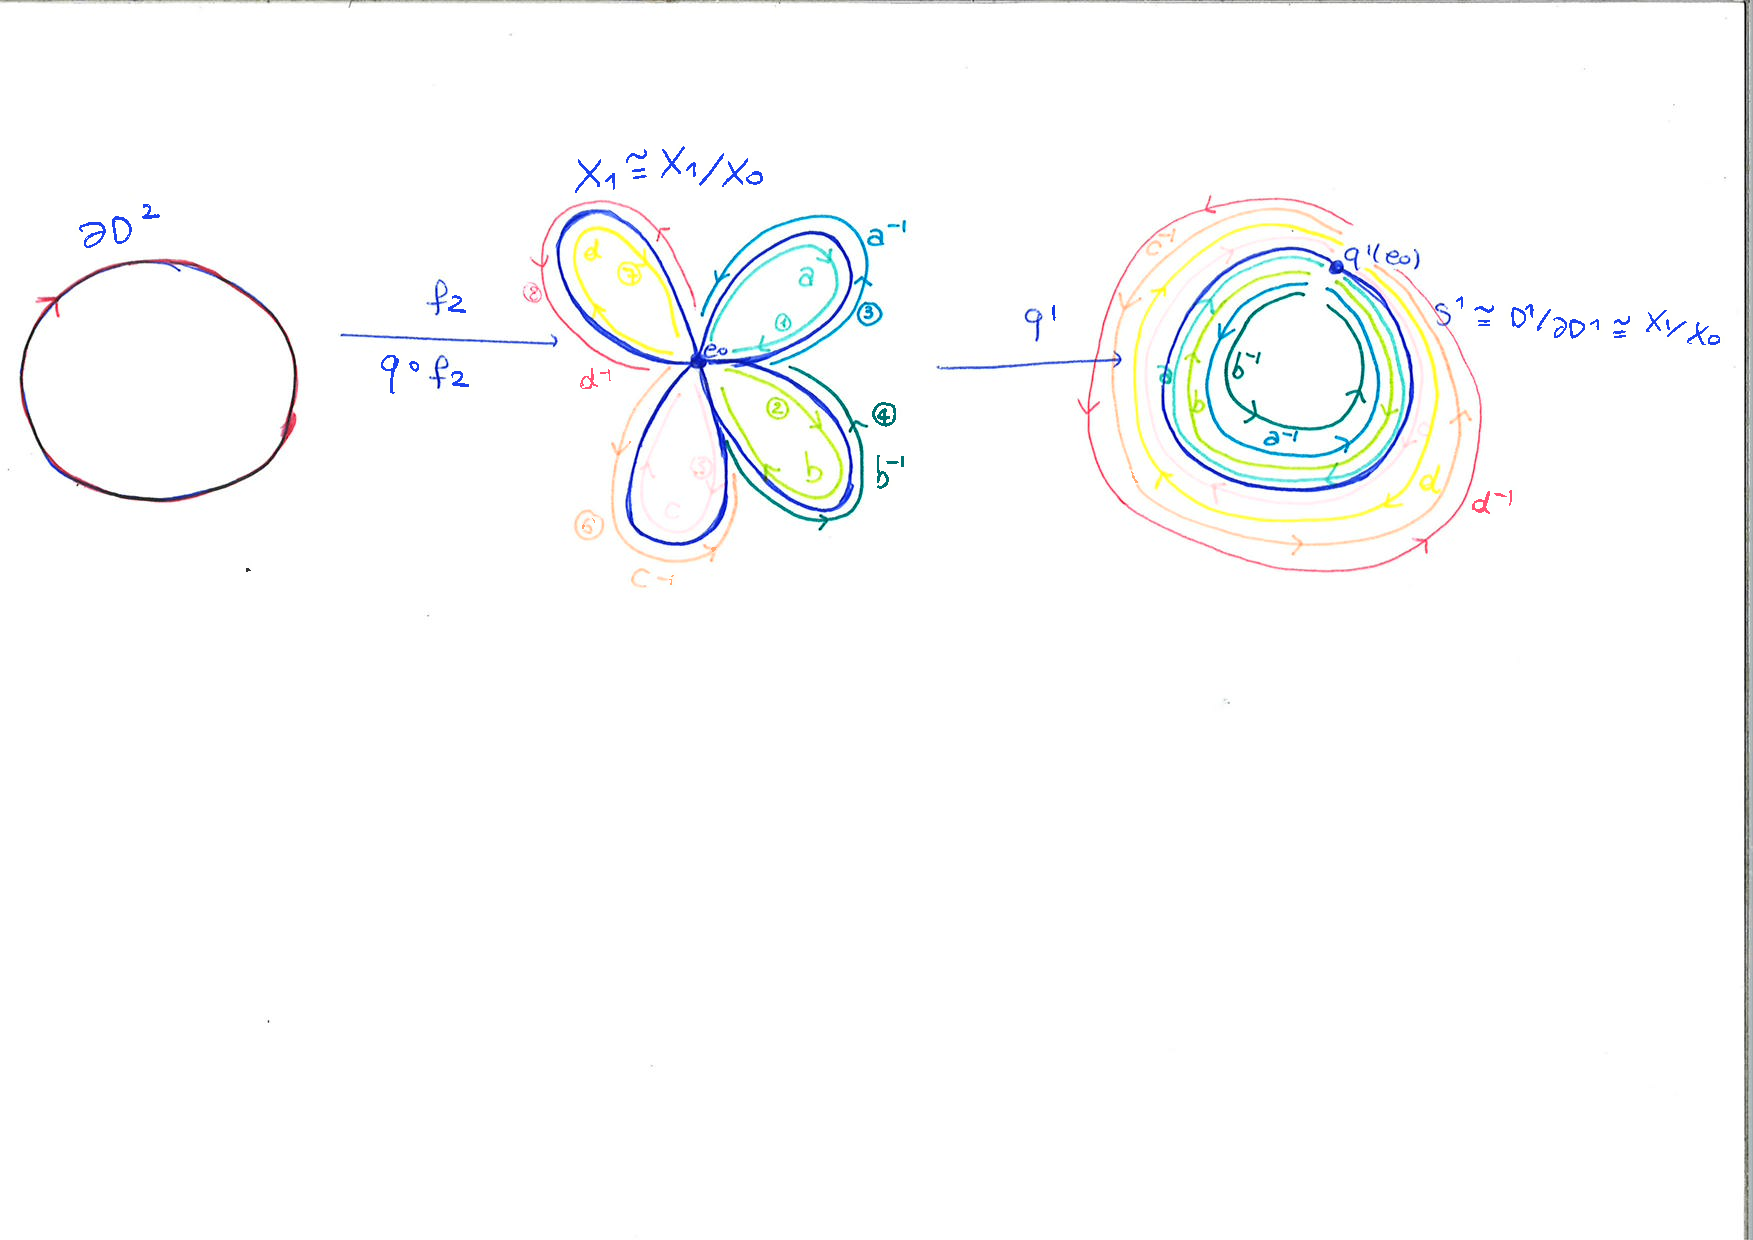
\includegraphics[width=\linewidth]{pic1ass8at1.pdf}
\end{figure}
It follows that, in $\tilde{\partial}_2(e^2)$, the coefficients are all 0, thus $\tilde{\partial}_2$ is the zero-map and $H_2(X,\Z)\cong H_2(\tilde{C}(X,\Z))\cong\Z$, $H_1(X,\Z)\cong H_1(\tilde{C}(X,\Z))\cong\Z^4$

$(b)$ This surface is a torus of genus 2.

\newpage
\exercise{10.1}

First, we prove that $\varinjlim S^n\cong S^{\infty}$, where the maps are the inclusions $S^m\xrightarrow{i_{mn}} S^n$.

First of all, we see that the inclusion maps $S^n\xrightarrow{i_n} S^{\infty}$ are s.t. their diagram commutes, as $i_n\circ i_{mn}(x_0,\ldots,x_m)=(x_0,\ldots,x_m,0,\ldots,0)=i_m(x_0,\ldots,x_m)$.
\[
  \begin{tikzcd}
    S^m\arrow{rr}{i_{mn}}\arrow[swap]{dr}{f_m} & & S^m\arrow{dl}{f_n} \\
    & X
  \end{tikzcd}
\]
Now, let $S^n\xrightarrow{f_n} X$ be a collection of maps s.t. the diagram commutes. Then, we may construct $S^{\infty}\xrightarrow{f} X$ by setting, for some $(x_i)_{i\in\N}$, $f((x_i)_{i\in\N})=f_n(x_0,\ldots,x_n)$, where $n$ is s.t. $x_m=0$ for all $m>n$. It is well defined: indeed, taking another $m$ with the same property as $n$, assuming that $m>n$, we see that $f_n(x_0,\ldots,x_n)=f_m\circ i_{nm}(x_0,\ldots,x_n)=f_m(x_0,\ldots,x_n,0,\ldots,0)=f_m(x_0,\ldots,x_m)$ by the commutativity and the fact that $x_i=0$ for $i>n$, hence we are done. The same happens if $n>m$ and the proof is essentially identical.

By construction, $f\circ i_n(x_0,\ldots,x_n)=f_n(x_0,\ldots,x_n)$, hence we are done if we can prove that $f$ is continuous, which follows from the fact that $S^n\cap f^{-1}(U)=f^{-1}_n(U)$, which is open for every $n$ by continuity of $f_n$. The uniqueness follows from the fact that an $f'$ making the diagram commute has to be s.t. $f'\circ i_n=f_n=f\circ i_n$ for every $n$ and every point of $S^{\infty}$ lies in the image of some $i_n$.
\[
  \begin{tikzcd}
    S^m\arrow{rr}{i_{mn}}\arrow{dr}{i_m}\arrow[swap]{ddr}{f_m} & & S^n\arrow[swap]{dl}{i_n}\arrow{ddl}{f_n} \\
    & S^{\infty}\arrow{d}{f} \\
    & X
  \end{tikzcd}
\]
Now we show that the following diagram, where $\pi_n:S^n\rightarrow S^n_{/\sim}$ is the projection map and $j_{mn}:S^m_{/\sim}\rightarrow S^n_{/\sim}$ is defined as $j_{mn}([x_0,\ldots,x_m])=[x_0,\ldots,x_m,0\ldots,0]$ (which is again s.t. $j_{nk}\circ j_{mn}=j_{mk}$, as $j_{nk}\circ j_{mn}([x_0,\ldots,x_m])=[x_0,\ldots,x_m,0,\ldots,0]=j_{mk}([x_0,\ldots,x_m])$), commutes:
\[
  \begin{tikzcd}
    S^0\arrow{d}{\pi_0}\arrow{r}{i_{0,1}} & S^1\arrow{d}{\pi_1}\arrow{r}{i_{1,2}} & S^2\arrow{d}{\pi_2}\arrow{r}{i_{2,3}} & \cdots \\
    S^0_{/\sim}\arrow{r}{j_{0,1}} & S^1_{/\sim}\arrow{r}{j_{1,2}} & S^2_{/\sim}\arrow{r}{j_{2,3}} & \cdots
  \end{tikzcd}
\]

To do this, it is sufficient to show that the generic square of the following form commutes:
\[
  \begin{tikzcd}
    S^n\arrow{d}{\pi_n}\arrow{r}{i_{n,n+1}} & S^{n+1}\arrow{d}{\pi_{n+1}} \\
    S^n_{/\sim}\arrow{r}{j_{n,n+1}} & S^{n+1}_{/\sim}
  \end{tikzcd}
\]

This follows from the fact that $j_{n,n+1}\circ\pi_n(x_0,\ldots,x_n)=j_{n,n+1}([x_0,\ldots,x_n])=[x_0,\ldots,x_n,0]=\pi_{n+1}(x_0,\ldots,x_n,0)=\pi_{n+1}\circ i_{n,n+1}(x_0,\ldots,x_n)$.

Now we will show that $\varinjlim S^n_{/\sim}\cong S^{\infty}_{/\sim}$, where the map $i_n:S^n_{/\sim}\rightarrow S^{\infty}_{/\sim}$ is defined as $i_n([x_0,\ldots,x_n])=[(x_i)_{i\in\N}]$, where $x_i=0$ for $i>n$.

First of all, $i_n\circ i_{mn}([x_0,\ldots,x_m])=i_n([x_0,\ldots,x_m,0,\ldots,0])=[(x_i)_{i\in\N}]=i_m([x_0,\ldots,x_m])$, where $x_i=0$ for $i>m$ by construction.
\[
  \begin{tikzcd}
    S^m\arrow{d}{\pi_m}\arrow{rr}{i_{mn}} & & S^n\arrow{d}{\pi_n} \\
    S^m_{/\sim}\arrow{rr}{j_{mn}}\arrow[swap]{dr}{g_m} & & S^n_{/\sim}\arrow{dl}{g_n} \\
    & X
\end{tikzcd}
\]
Let $S^n_{/\sim}\xrightarrow{g_n} X$ be a collection of maps s.t. the diagram commutes. Then, we may lift each of them through the $\pi_n$ to maps on $S^n$, let's say $f_n$, defined as $f_n:=g_n\circ\pi_n$, i.e. $f_n(x_0,\ldots,x_n)=g_n([x_0,\ldots,x_n])$. By construction, $f_m(x_0,\ldots,x_m)=g_m([x_0,\ldots,x_m])=g_n\circ j_{mn}([x_0,\ldots,x_m])=g_n([x_0,\ldots,x_m,0,\ldots,0])=f_n(x_0,\ldots,x_m,0,\ldots,0)=f_n\circ i_{mn}(x_0,\ldots,x_m)$, hence they make the diagram commute. It follows that there is a unique $f:S^{\infty}\rightarrow X$ s.t. $f\circ i_n=f_n$ and it is defined as before.

Again, by construction, $f((x_i)_{i\in\N})=f_n(x_0,\ldots,x_n)=g_n([x_0,\ldots,x_n])=g_n([-x_0,\ldots,-x_n])=f_n(-x_0,\ldots,-x_n)=f((-x_i)_{i\in\N})$, thus $f$ is uniquely factorized through the quotient map $\pi_{\infty}:S^{\infty}\rightarrow S^{\infty}_{/\sim}$, inducing a unique continuous map $g:S^{\infty}_{/\sim}\rightarrow X$.

The thesis follows, as $g\circ j_n\circ\pi_n=g\circ \pi_{\infty}\circ i_n=f\circ i_n=f_n=g_n\circ\pi_n$ because $j_n\circ\pi_n(x_0,\ldots,x_n)=j_n([x_0,\ldots,x_n])=[(x_i)_{i\in\N}]=\pi_{\infty}((x_i)_{i\in\N})=\pi_{\infty}\circ i_n(x_0,\ldots,x_n)$, where $x_i=0$ for $i>n$, and each projection is an epimorphism, thus $g\circ j_n=g_n$ and the diagram commutes.
\[
  \begin{tikzcd}
    S^m_{/\sim}\arrow{rr}{j_{mn}}\arrow{dr}{j_m}\arrow[swap]{ddr}{g_m} & & S^n_{/\sim}\arrow[swap]{dl}{i_n}\arrow{ddl}{g_n} \\
    & S^{\infty}_{/\sim}\arrow{d}{g} \\
    & X
  \end{tikzcd}
\]

Consider the canonical inclusions $j'_{mn}:\Ps^m_{\R}\rightarrow\Ps^n_{\R}$ used to construct each $\Ps^n_{\R}$ as a CW-complex and the usual homeomorphisms $\phi:S^n_{/\sim}\rightarrow\Ps^n_{\R}$. We want to show that the following diagram commutes:
\[
  \begin{tikzcd}
    S^0_{/\sim}\arrow{r}{j_{0,1}}\arrow{d}{\phi_0} & S^1_{/\sim}\arrow{r}{j_{1,2}}\arrow{d}{\phi_1} & S^2_{/\sim}\arrow{r}{j_{2,3}}\arrow{d}{\phi_2} & \cdots \\
    \Ps^0_{\R}\arrow{r}{j'_{0,1}} & \Ps^1_{\R}\arrow{r}{j'_{1,2}} & \Ps^2_{\R}\arrow{r}{j'_{2,3}} & \cdots
  \end{tikzcd}
\]

Again, we only have to show it for a generic square of the following form:
\[
  \begin{tikzcd}
    S^n_{/\sim}\arrow{r}{j_{n,n+1}}\arrow{d}{\phi_n} & S^{n+1}_{/\sim}\arrow{d}{\phi_{n+1}} \\
    \Ps^n_{\R}\arrow{r}{j'_{n,n+1}} & \Ps^{n+1}_{\R}
  \end{tikzcd}
\]
We see that $j'_{mn}\circ\phi_m([x_0,\ldots,x_m])=j'_{mn}([x_0:\ldots:x_m])=[x_0:\ldots:x_m:0:\ldots:0]=\phi_n([x_0,\ldots,x_n,0,\ldots,0])=\phi_n\circ j_{mn}([x_0,\ldots,x_n])$, hence we are done.

Now we have induced on each $S^n$ a CW-complex structure which is compatible with the maps, as the following diagram shows (remember that in a commutative square we may reverse all of the isomorphisms and still have a commutative square):
\[
  \begin{tikzcd}
    \partial D^{n+1}\arrow{d}\arrow{r}\arrow[bend left]{rr} & \Ps^n_{\R}\arrow[swap]{d}{j'_{n,n+1}}\arrow[swap]{r}{\phi_n^{-1}} & S^n_{/\sim}\arrow{d}{j_{n,n+1}} \\
    D^{n+1}\arrow{r}\arrow[bend right]{rr} & \Ps^{n+1}_{\R}\arrow{r}{\phi_{n+1}^{-1}} & S^{n+1}_{/\sim}
  \end{tikzcd}
\]

In particular, since a succession of finite CW-complexes where $X_{n+1}$ is obtained by glueing to $X_n$ some $(n+1)$-cells is s.t. $\varinjlim X_n\cong X$, where $X=\bigcup_{n\in\N} X_n$ is again a CW-complex by construction, we have that $\varinjlim \Ps^n_{\R}$ exists and it is isomorphic (homeomorphic) to $\varinjlim S^n_{/\sim}\cong S^{\infty}_{/\sim}$, as the two chains are isomorphic and therefore their colimits are as well. We have therefore induced the desired CW-complex structure on $S^{\infty}_{/\sim}$.

We shall now compute $H_n(S^{\infty}_{/\sim},\Z)$.

By~\cite[prop. 9.12]{sag}, we know that $H_n(S^{\infty}_{/\sim},\Z)\cong H_n(S^{n+1}_{/\sim},\Z)\cong H_n(\Ps^{n+1}_{\R},\Z)$. By~\cite[thm. 10.9]{sag}, we can conclude that:
$$
  H_n(S^{\infty}_{/\sim},\Z)\cong\begin{cases}
    \F_2\textit{ if $n$ is odd} \\
    0\textit{ otherwise}
  \end{cases}
$$



\begin{thebibliography}{9}
  \bibitem{sag}
    S. Sagave,
    \textit{Algebraic Topology},
    2017
\end{thebibliography}

\end{document}
